\documentclass[tikz,border=5pt]{standalone}

\usepackage[T1]{fontenc}
\usepackage{lmodern}
\usepackage{xcolor}
\usetikzlibrary{arrows.meta,positioning,calc,fit,backgrounds}

\definecolor{ink}{HTML}{0F172A}
\definecolor{muted}{HTML}{475569}
\definecolor{line}{HTML}{CBD5E1}
\definecolor{panel}{HTML}{F8FAFC}
\definecolor{blue}{HTML}{2563EB}
\definecolor{cyan}{HTML}{0D9488}
\definecolor{amber}{HTML}{D97706}
\definecolor{green}{HTML}{059669}
\definecolor{rose}{HTML}{E11D48}

\begin{document}
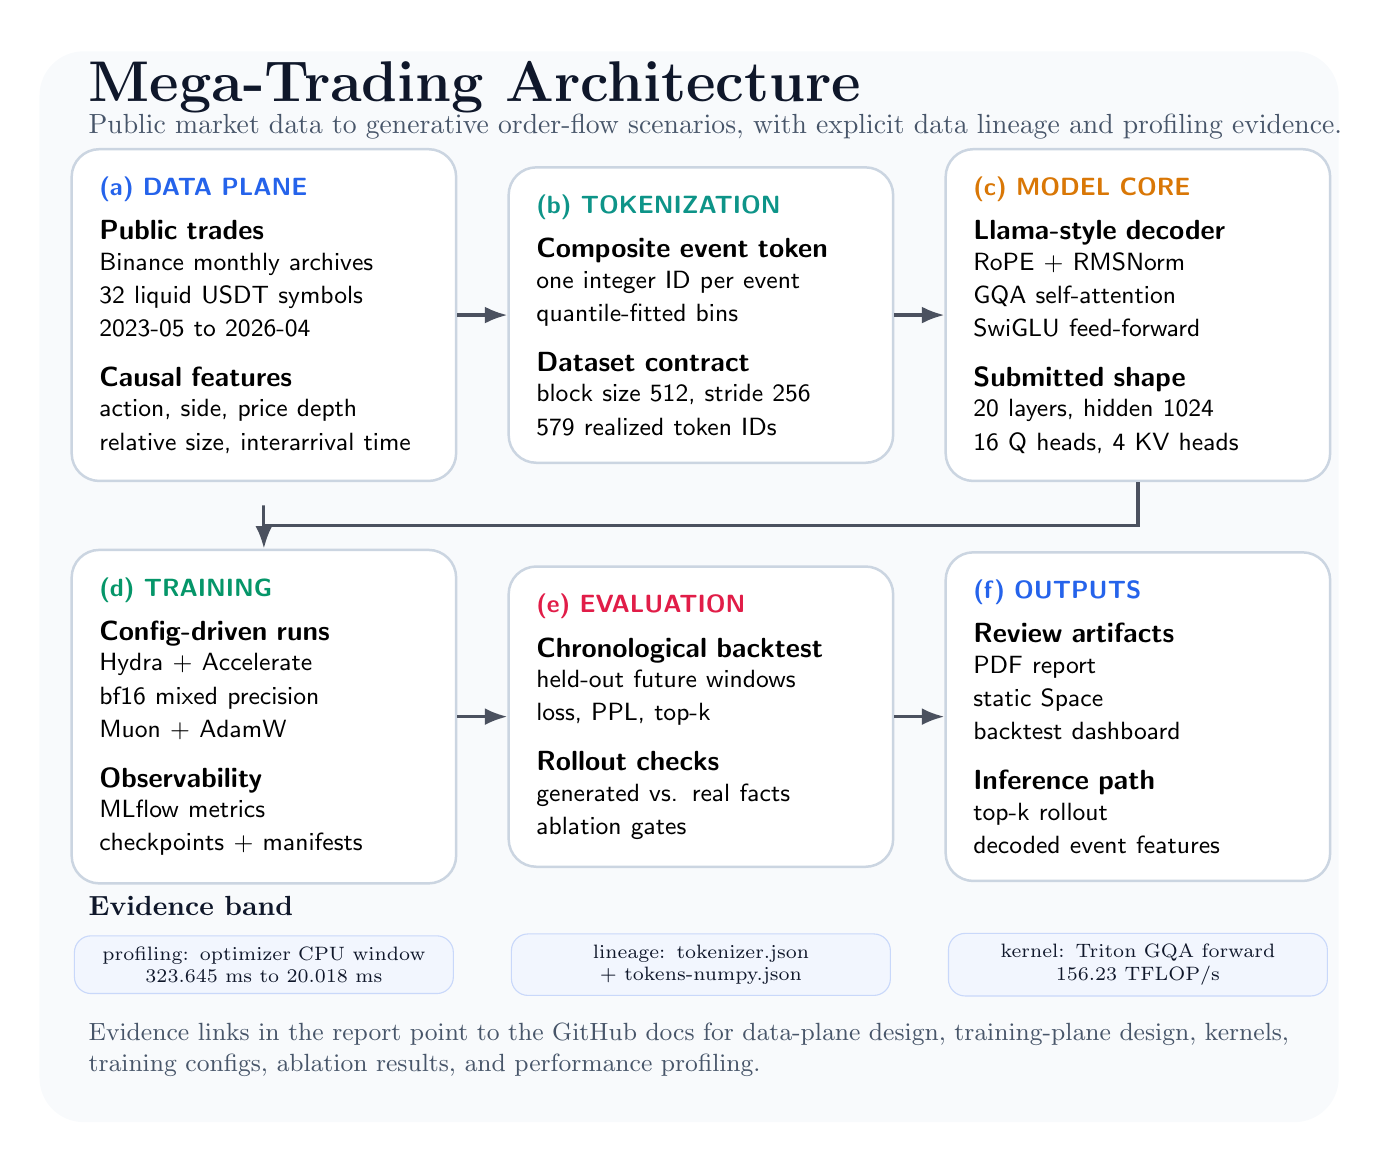
\begin{tikzpicture}[
  font=\sffamily,
  >=Latex,
  stage/.style={
    draw=line,
    rounded corners=10pt,
    fill=white,
    line width=0.9pt,
    minimum width=4.75cm,
    minimum height=2.85cm,
    text width=4.18cm,
    align=left,
    inner sep=10pt
  },
  header/.style={font=\bfseries\small, text=blue},
  title/.style={font=\bfseries\normalsize, text=ink},
  body/.style={font=\small, text=muted},
  metric/.style={font=\bfseries\scriptsize, text=ink},
  chip/.style={
    rounded corners=6pt,
    draw=blue!25,
    fill=blue!6,
    text width=4.25cm,
    minimum height=0.62cm,
    align=center,
    inner xsep=8pt,
    inner ysep=4pt,
    font=\scriptsize,
    text=ink
  },
  link/.style={->, line width=1.15pt, draw=ink!75},
  evidence/.style={->, line width=0.95pt, draw=blue!80, dashed}
]

\path[use as bounding box] (-0.70,-1.05) rectangle (16.20,13.10);
\fill[panel, rounded corners=16pt] (-0.55,-0.80) rectangle (15.95,12.80);
\node[anchor=west, font=\bfseries\huge, text=ink] at (-0.05,12.35)
  {Mega-Trading Architecture};
\node[anchor=west, font=\normalsize, text=muted] at (-0.05,11.85)
  {Public market data to generative order-flow scenarios, with explicit data lineage and profiling evidence.};

\node[stage] (data) at (2.30,9.45) {
  \textcolor{blue}{\textbf{\small (a) DATA PLANE}}\\[4pt]
  \textbf{\normalsize Public trades}\\[-1pt]
  {\small Binance monthly archives}\\
  {\small 32 liquid USDT symbols}\\
  {\small 2023-05 to 2026-04}\\[6pt]
  \textbf{\normalsize Causal features}\\[-1pt]
  {\small action, side, price depth}\\
  {\small relative size, interarrival time}
};

\node[stage] (token) at (7.85,9.45) {
  \textcolor{cyan}{\textbf{\small (b) TOKENIZATION}}\\[4pt]
  \textbf{\normalsize Composite event token}\\[-1pt]
  {\small one integer ID per event}\\
  {\small quantile-fitted bins}\\[6pt]
  \textbf{\normalsize Dataset contract}\\[-1pt]
  {\small block size 512, stride 256}\\
  {\small 579 realized token IDs}
};

\node[stage] (model) at (13.40,9.45) {
  \textcolor{amber}{\textbf{\small (c) MODEL CORE}}\\[4pt]
  \textbf{\normalsize Llama-style decoder}\\[-1pt]
  {\small RoPE + RMSNorm}\\
  {\small GQA self-attention}\\
  {\small SwiGLU feed-forward}\\[6pt]
  \textbf{\normalsize Submitted shape}\\[-1pt]
  {\small 20 layers, hidden 1024}\\
  {\small 16 Q heads, 4 KV heads}
};

\node[stage] (train) at (2.30,4.35) {
  \textcolor{green}{\textbf{\small (d) TRAINING}}\\[4pt]
  \textbf{\normalsize Config-driven runs}\\[-1pt]
  {\small Hydra + Accelerate}\\
  {\small bf16 mixed precision}\\
  {\small Muon + AdamW}\\[6pt]
  \textbf{\normalsize Observability}\\[-1pt]
  {\small MLflow metrics}\\
  {\small checkpoints + manifests}
};

\node[stage] (eval) at (7.85,4.35) {
  \textcolor{rose}{\textbf{\small (e) EVALUATION}}\\[4pt]
  \textbf{\normalsize Chronological backtest}\\[-1pt]
  {\small held-out future windows}\\
  {\small loss, PPL, top-k}\\[6pt]
  \textbf{\normalsize Rollout checks}\\[-1pt]
  {\small generated vs. real facts}\\
  {\small ablation gates}
};

\node[stage] (serve) at (13.40,4.35) {
  \textcolor{blue}{\textbf{\small (f) OUTPUTS}}\\[4pt]
  \textbf{\normalsize Review artifacts}\\[-1pt]
  {\small PDF report}\\
  {\small static Space}\\
  {\small backtest dashboard}\\[6pt]
  \textbf{\normalsize Inference path}\\[-1pt]
  {\small top-k rollout}\\
  {\small decoded event features}
};

\draw[link] (data.east) -- (token.west);
\draw[link] (token.east) -- (model.west);
\draw[link] (model.south) -- ++(0,-0.55) -| ($(train.north)+(0,0.55)$) -- (train.north);
\draw[link] (train.east) -- (eval.west);
\draw[link] (eval.east) -- (serve.west);

\node[anchor=west, font=\bfseries\normalsize, text=ink] at (-0.05,1.95)
  {Evidence band};
\node[chip] (profile) at (2.30,1.20) {profiling: optimizer CPU window\\323.645 ms to 20.018 ms};
\node[chip] (lineage) at (7.85,1.20) {lineage: tokenizer.json\\+ tokens-numpy.json};
\node[chip] (kernel) at (13.40,1.20) {kernel: Triton GQA forward\\156.23 TFLOP/s};

\node[anchor=west, font=\small, text=muted, text width=15.4cm] at (-0.05,0.12)
  {Evidence links in the report point to the GitHub docs for data-plane design, training-plane design, kernels, training configs, ablation results, and performance profiling.};

\end{tikzpicture}
\end{document}
